\section{high.cpp File Reference}
\label{high_8cpp}\index{high.cpp@{high.cpp}}
{\tt \#include $<$iostream$>$}\par
{\tt \#include $<$fstream$>$}\par
{\tt \#include $<$iomanip$>$}\par
{\tt \#include \char`\"{}data\-In.h\char`\"{}}\par
{\tt \#include \char`\"{}high.h\char`\"{}}\par


Include dependency graph for high.cpp:\begin{figure}[H]
\begin{center}
\leavevmode
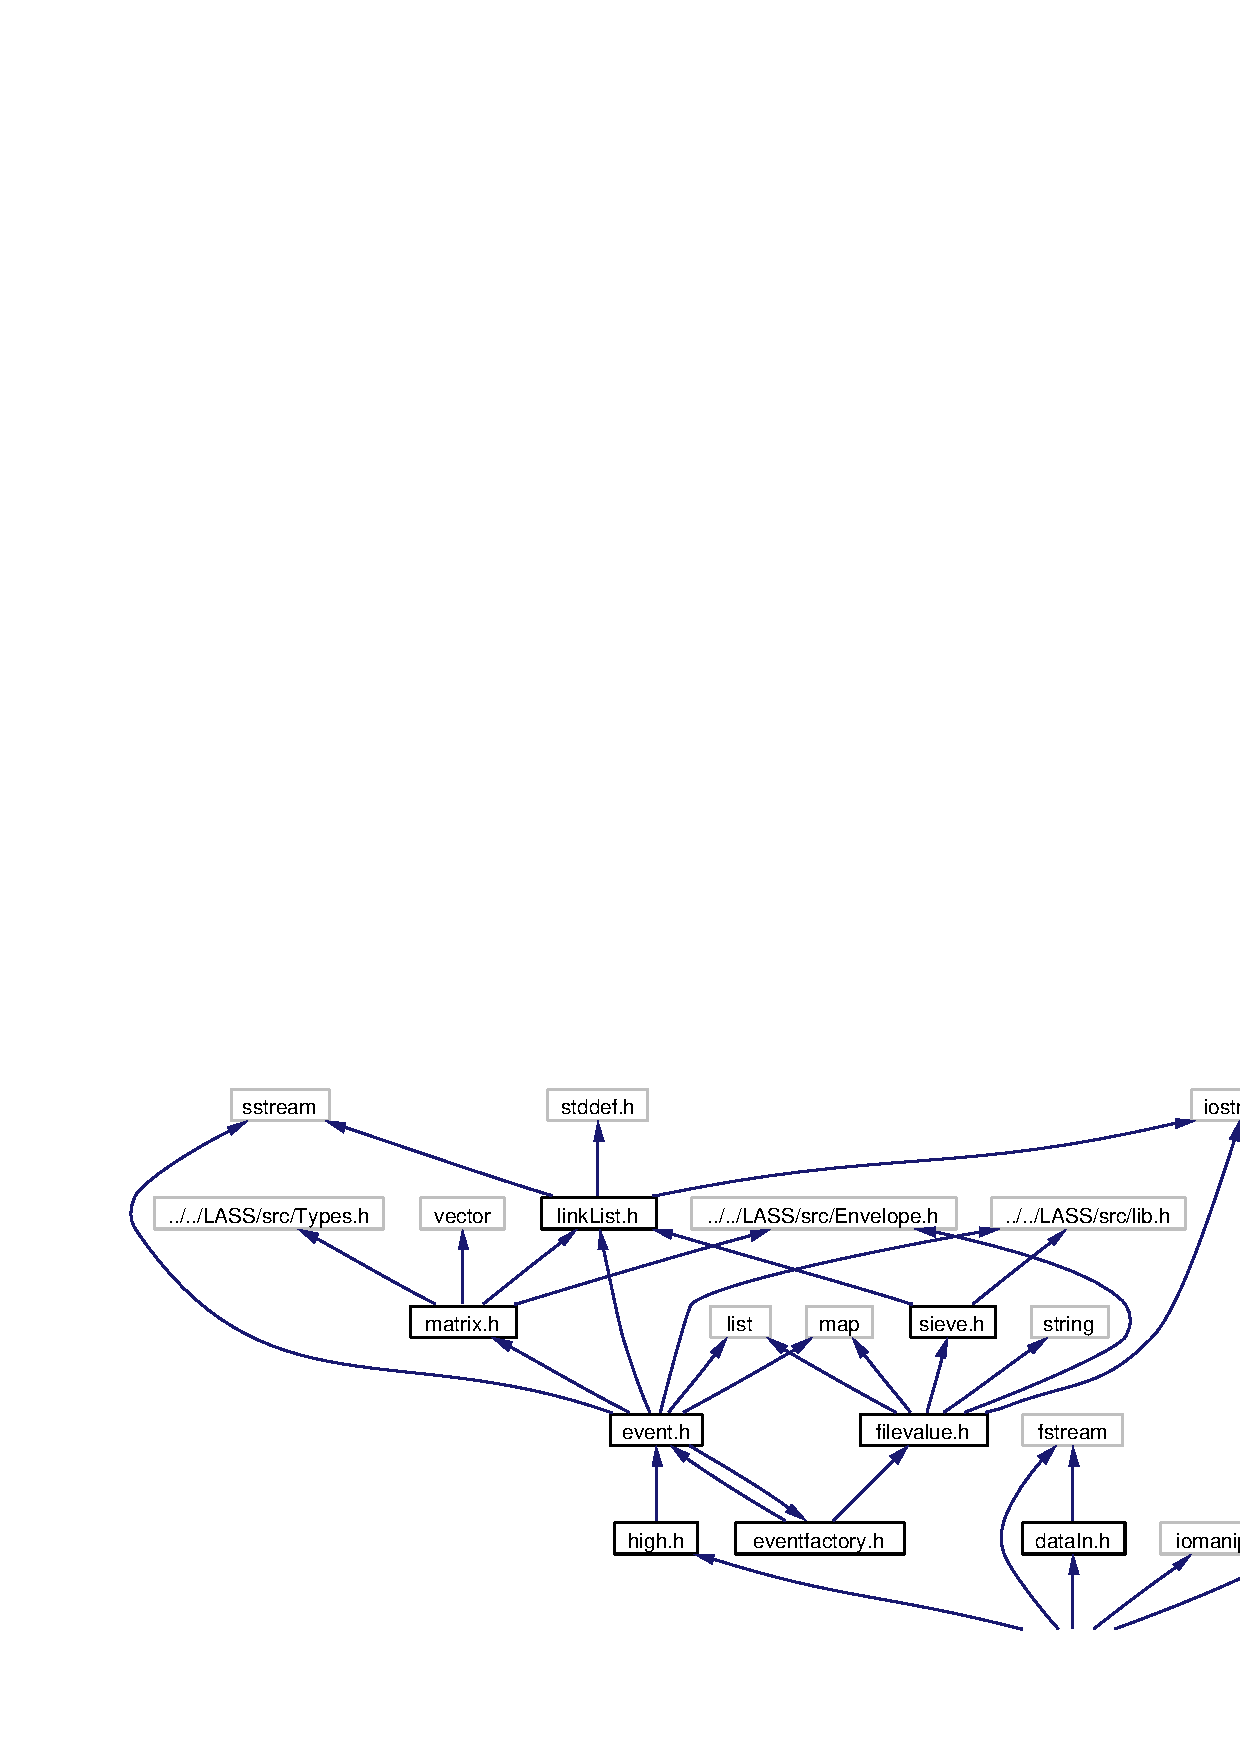
\includegraphics[width=323pt]{high_8cpp__incl}
\end{center}
\end{figure}
\subsection*{Variables}
\begin{CompactItemize}
\item 
ofstream $\ast$ {\bf output\-File}
\item 
int {\bf low\-ID}
\item 
int {\bf high\-ID}
\item 
int {\bf bottom\-ID}
\end{CompactItemize}


\subsection{Variable Documentation}
\index{high.cpp@{high.cpp}!bottomID@{bottomID}}
\index{bottomID@{bottomID}!high.cpp@{high.cpp}}
\subsubsection{\setlength{\rightskip}{0pt plus 5cm}int {\bf bottom\-ID}}\label{high_8cpp_a3}




Definition at line 36 of file high.cpp.\index{high.cpp@{high.cpp}!highID@{highID}}
\index{highID@{highID}!high.cpp@{high.cpp}}
\subsubsection{\setlength{\rightskip}{0pt plus 5cm}int {\bf high\-ID}}\label{high_8cpp_a2}




Definition at line 35 of file high.cpp.

Referenced by High::High(), and High::Print().\index{high.cpp@{high.cpp}!lowID@{lowID}}
\index{lowID@{lowID}!high.cpp@{high.cpp}}
\subsubsection{\setlength{\rightskip}{0pt plus 5cm}int {\bf low\-ID}}\label{high_8cpp_a1}




Definition at line 34 of file high.cpp.

Referenced by High::High(), Low::Low(), and Low::Print().\index{high.cpp@{high.cpp}!outputFile@{outputFile}}
\index{outputFile@{outputFile}!high.cpp@{high.cpp}}
\subsubsection{\setlength{\rightskip}{0pt plus 5cm}ofstream$\ast$ {\bf output\-File}}\label{high_8cpp_a0}




Definition at line 32 of file high.cpp.